\paragraph{Signatures including a Z boson}

\subparagraph{Mono-Z (leptonic) signature}

\begin{table}
\centering
\caption{Event selection requirements for the analysis of the Mono-Z signature with leptonic Z decays.
        The requirements are inspired to follow those used in typical experimental analyses.}
\begin{tabular}{c | c |r l}
Selection stage & Quantity & Requirement \\\hline


\multirow{ 2}{*}{Inclusive}         & lepton $\left|\eta\right|$                    & $< 2.5$ \\
                                    & leading (trailing) lepton \pt                 & $> 25 (20)$ GeV \\\hline

\multirow{ 2}{*}{Preselection}      & $\left|m_{ll}-m_{Z,\mathrm{nominal}}\right|$  & $< 15$ GeV\\
                                    & \MET                                          & $> 40$ GeV \\\hline

\multirow{ 3}{*}{Final selection}   & $\Delta\Phi(ll,\MET)$                         & $>2.7$\\
                                    &$|p_{T,ll} - \MET|/p_{T,ll}$                   & $<0.4$\\
                                    &  $\Delta R(ll)$                               & $<1.8$\\
                                    &  \MET                                         & $>80$ GeV \\ 
\end{tabular}


\label{tab:monozll_selection}

\end{table}

Inclusive distributions of the invariant masses of the dilepton and $\chi\chi$ systems are shown in \autoref{fig:monoz_kin_inclusive} (before preselection). Independently of the parameters, the dilepton mass spectrum is centered at the Z peak, without any nonresonant contribution. The $M_{\chi\chi}$ distribution illustrates the signal contributions from different diagrams. For $\mA>\ma$, DM is dominantly produced from on-shell $a$ boson production. In the inverted mass region $\mA<\ma$, the situation is reversed, and $H$ diagrams dominate.

\begin{figure}
\centering
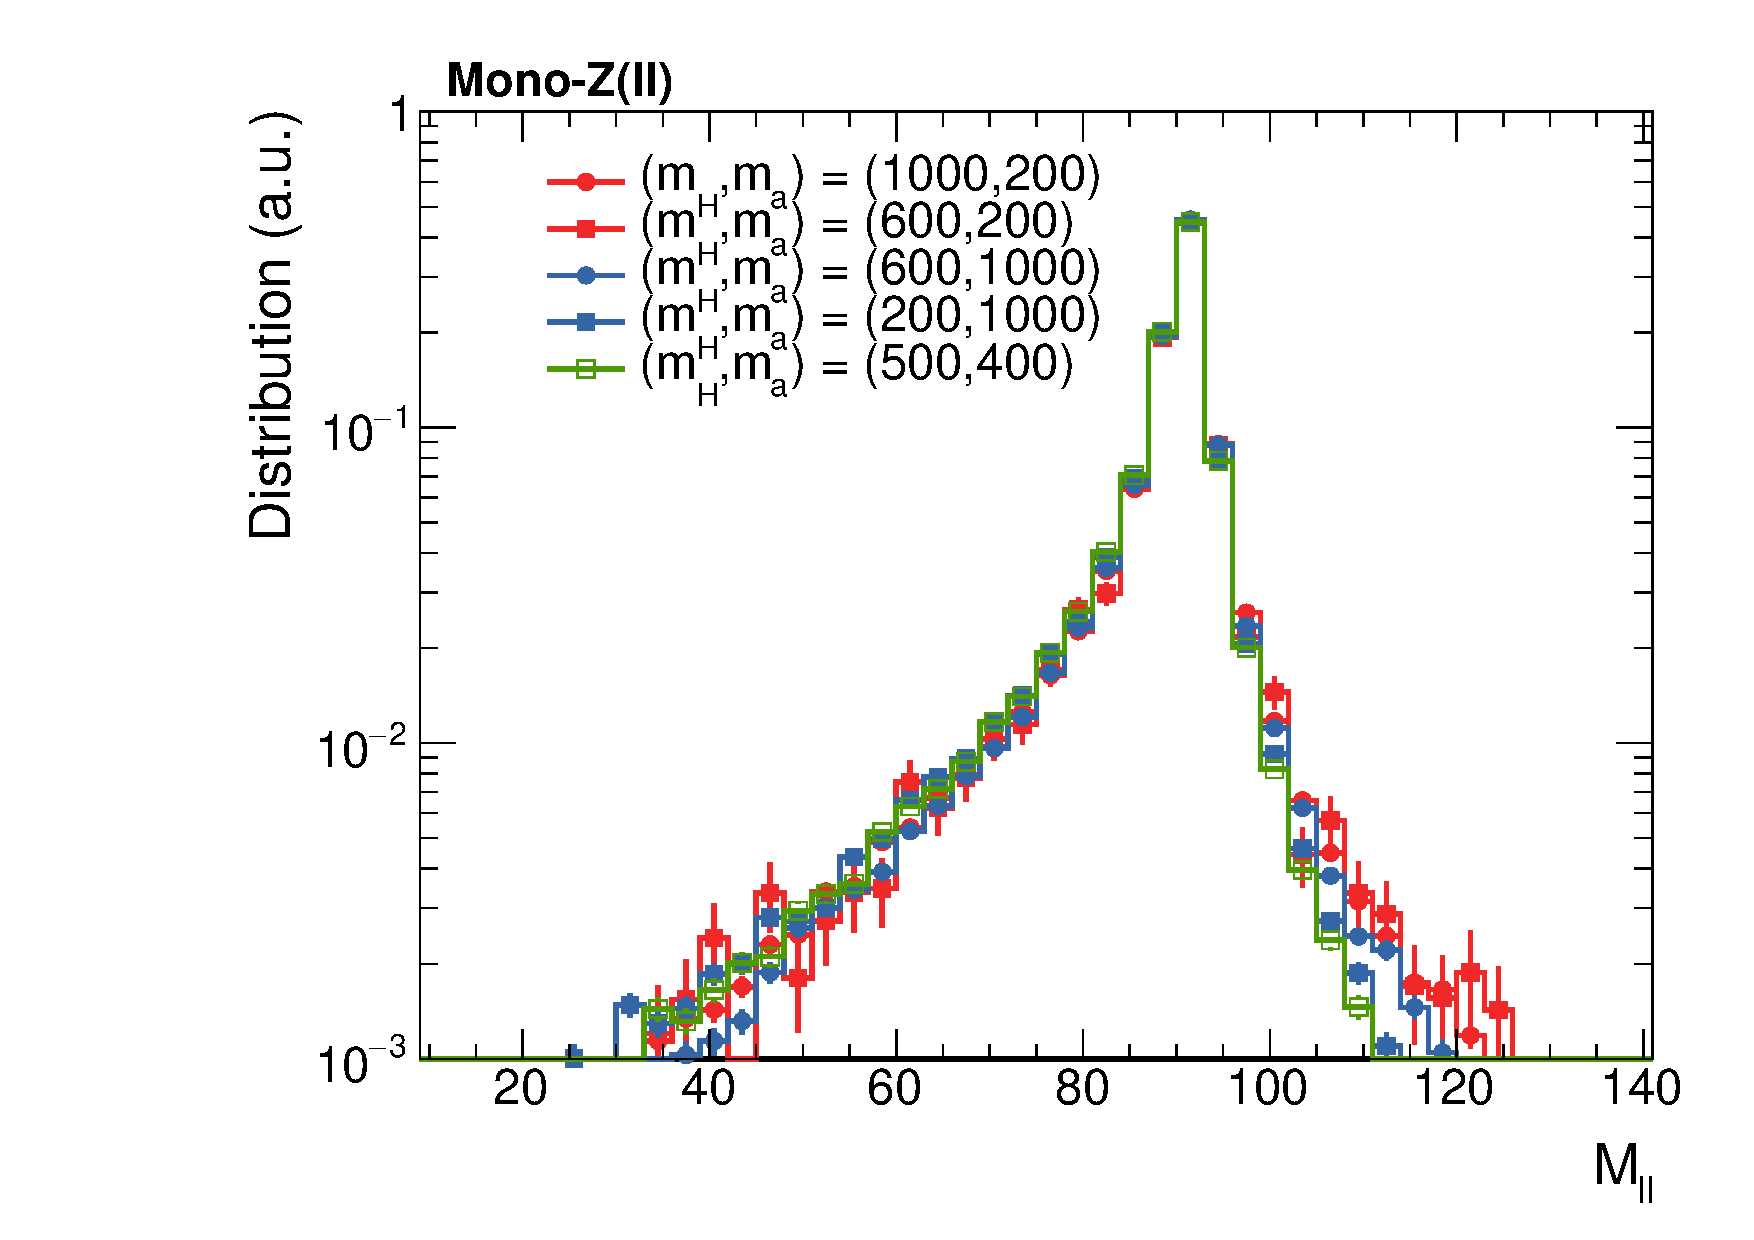
\includegraphics[width=0.45\textwidth]{texinputs/04_grid/figures/monoz/leptonic/inclusive_h_mz_lep.pdf}
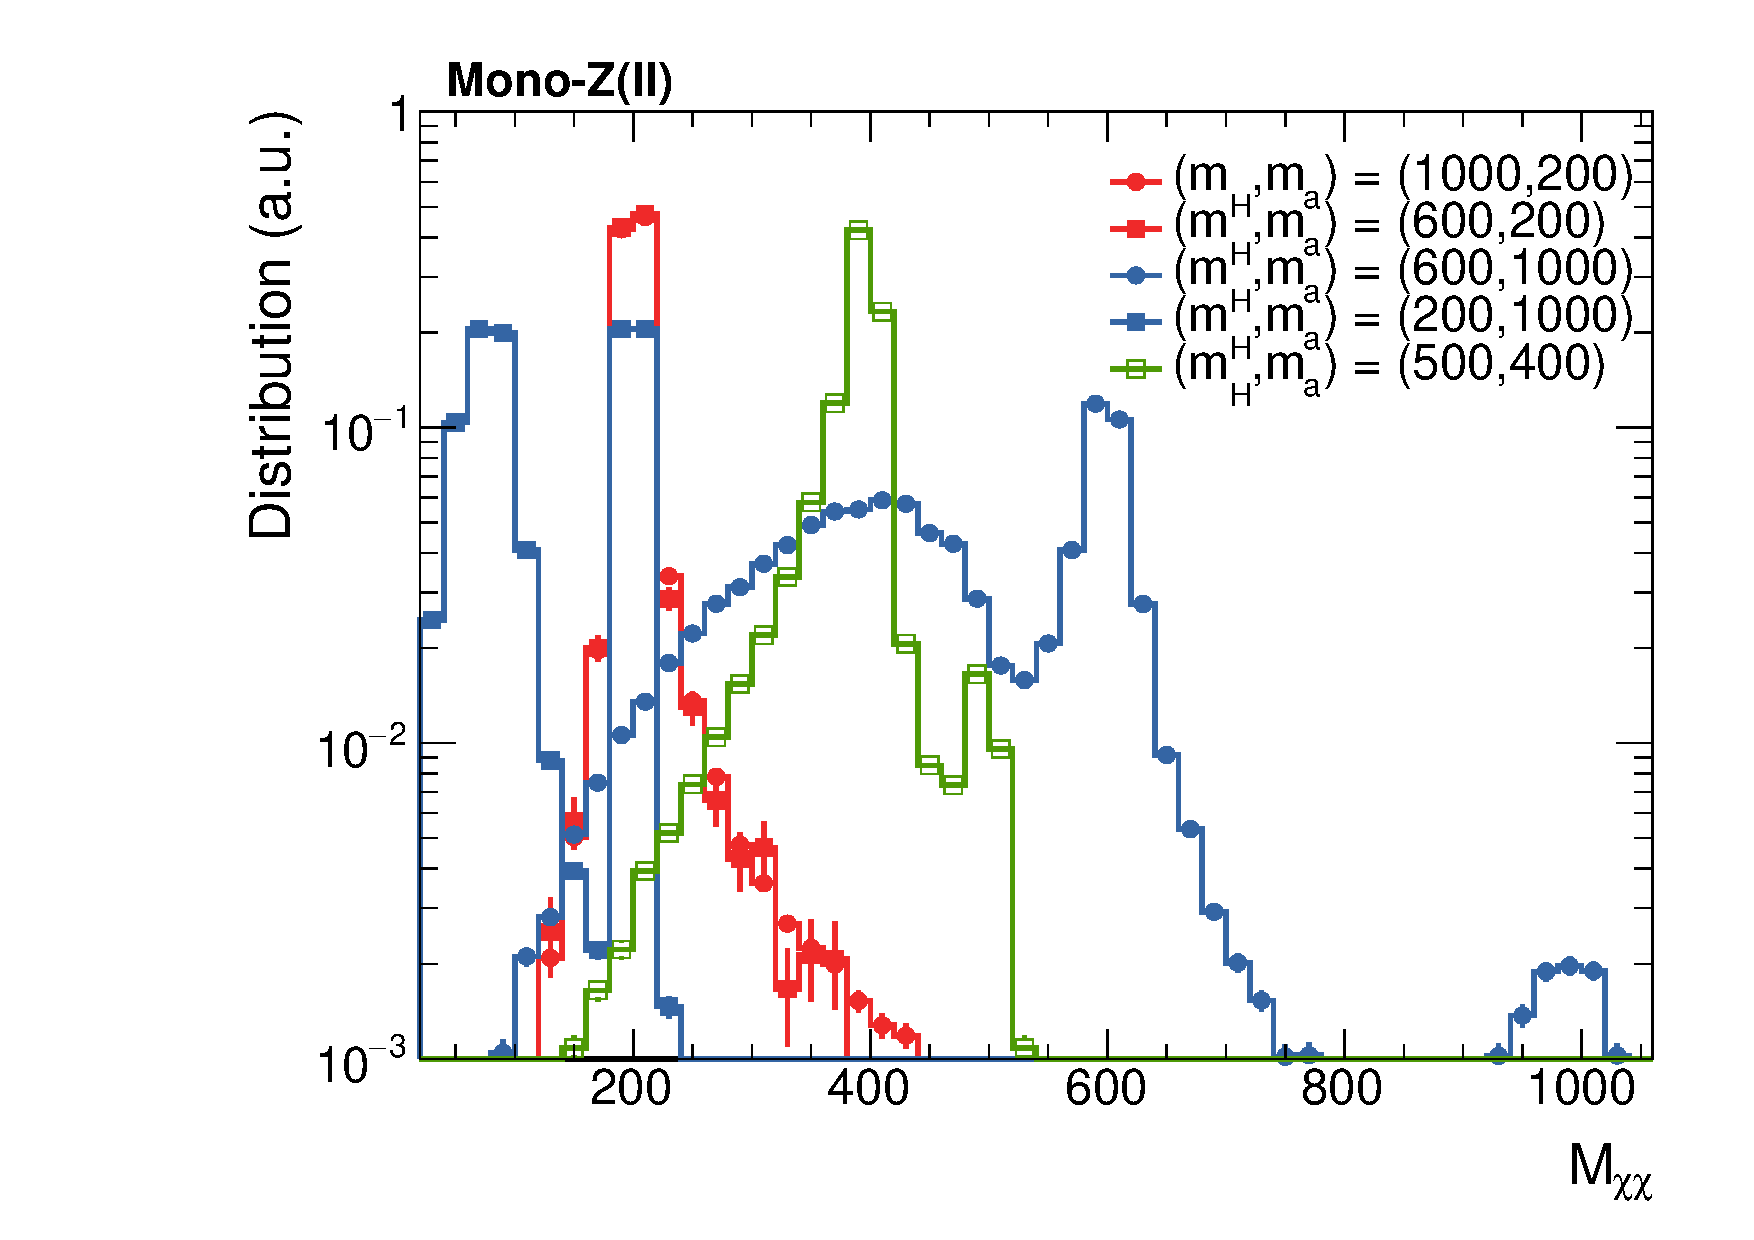
\includegraphics[width=0.45\textwidth]{texinputs/04_grid/figures/monoz/leptonic/inclusive_h_m_med_dm.pdf}
\caption{Distributions of the invariant mass of the dilepton (left) and $\chi\overline{\chi}$ systems (right) with no selection applied in addition to the generation cuts. The $M_{ll}$ distribution is centered around the Z boson mass independent of the chosen parameter point, indicating that there is no contribtion from $\gamma*$ exchange. The $M_{\chi\overline{\chi}}$ distribution }
\label{fig:monoz_kin_inclusive}
\end{figure}

The distributions of some relevant variables for this search are shown in \autoref{fig:monoz_kin_presel}, after preselection. 

\begin{figure}
\centering
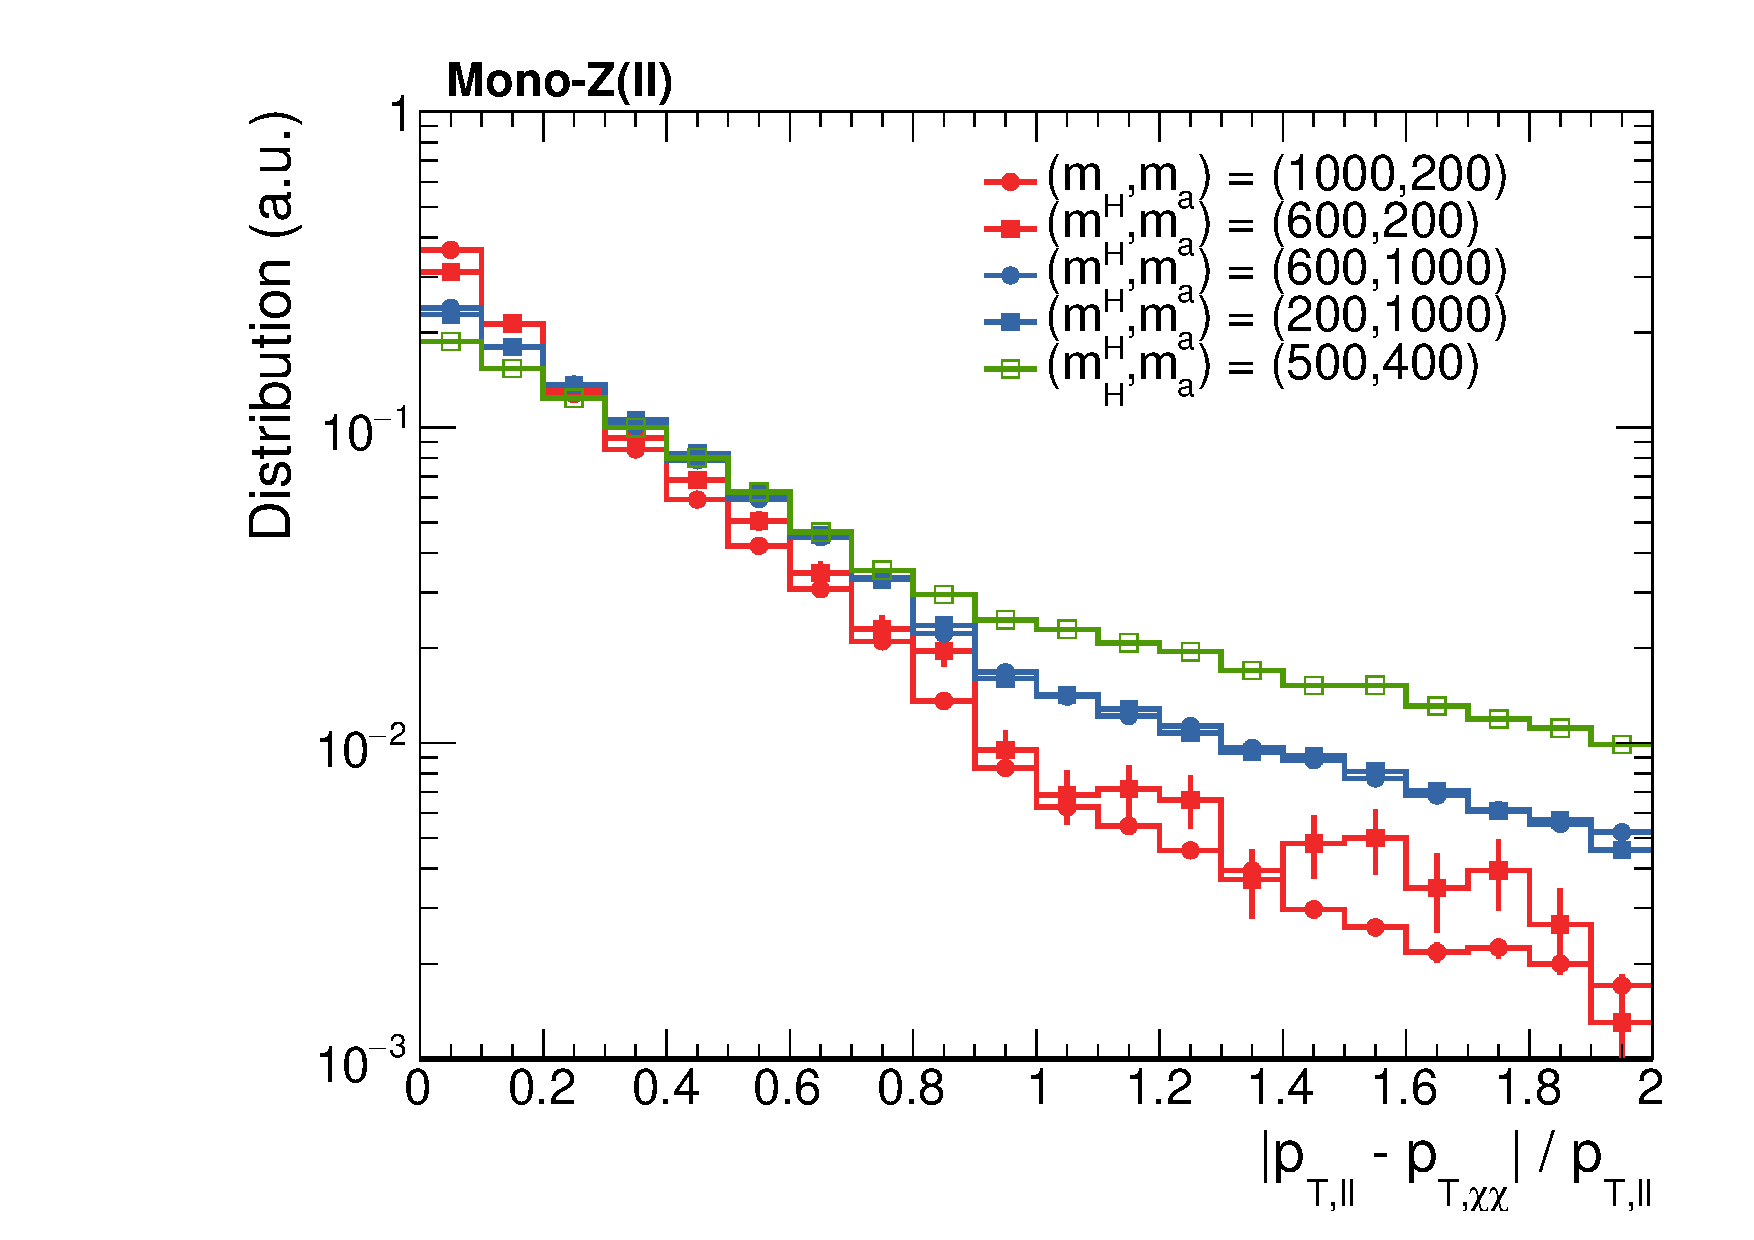
\includegraphics[width=0.45\textwidth]{texinputs/04_grid/figures/monoz/leptonic/presel_h_balance.pdf}
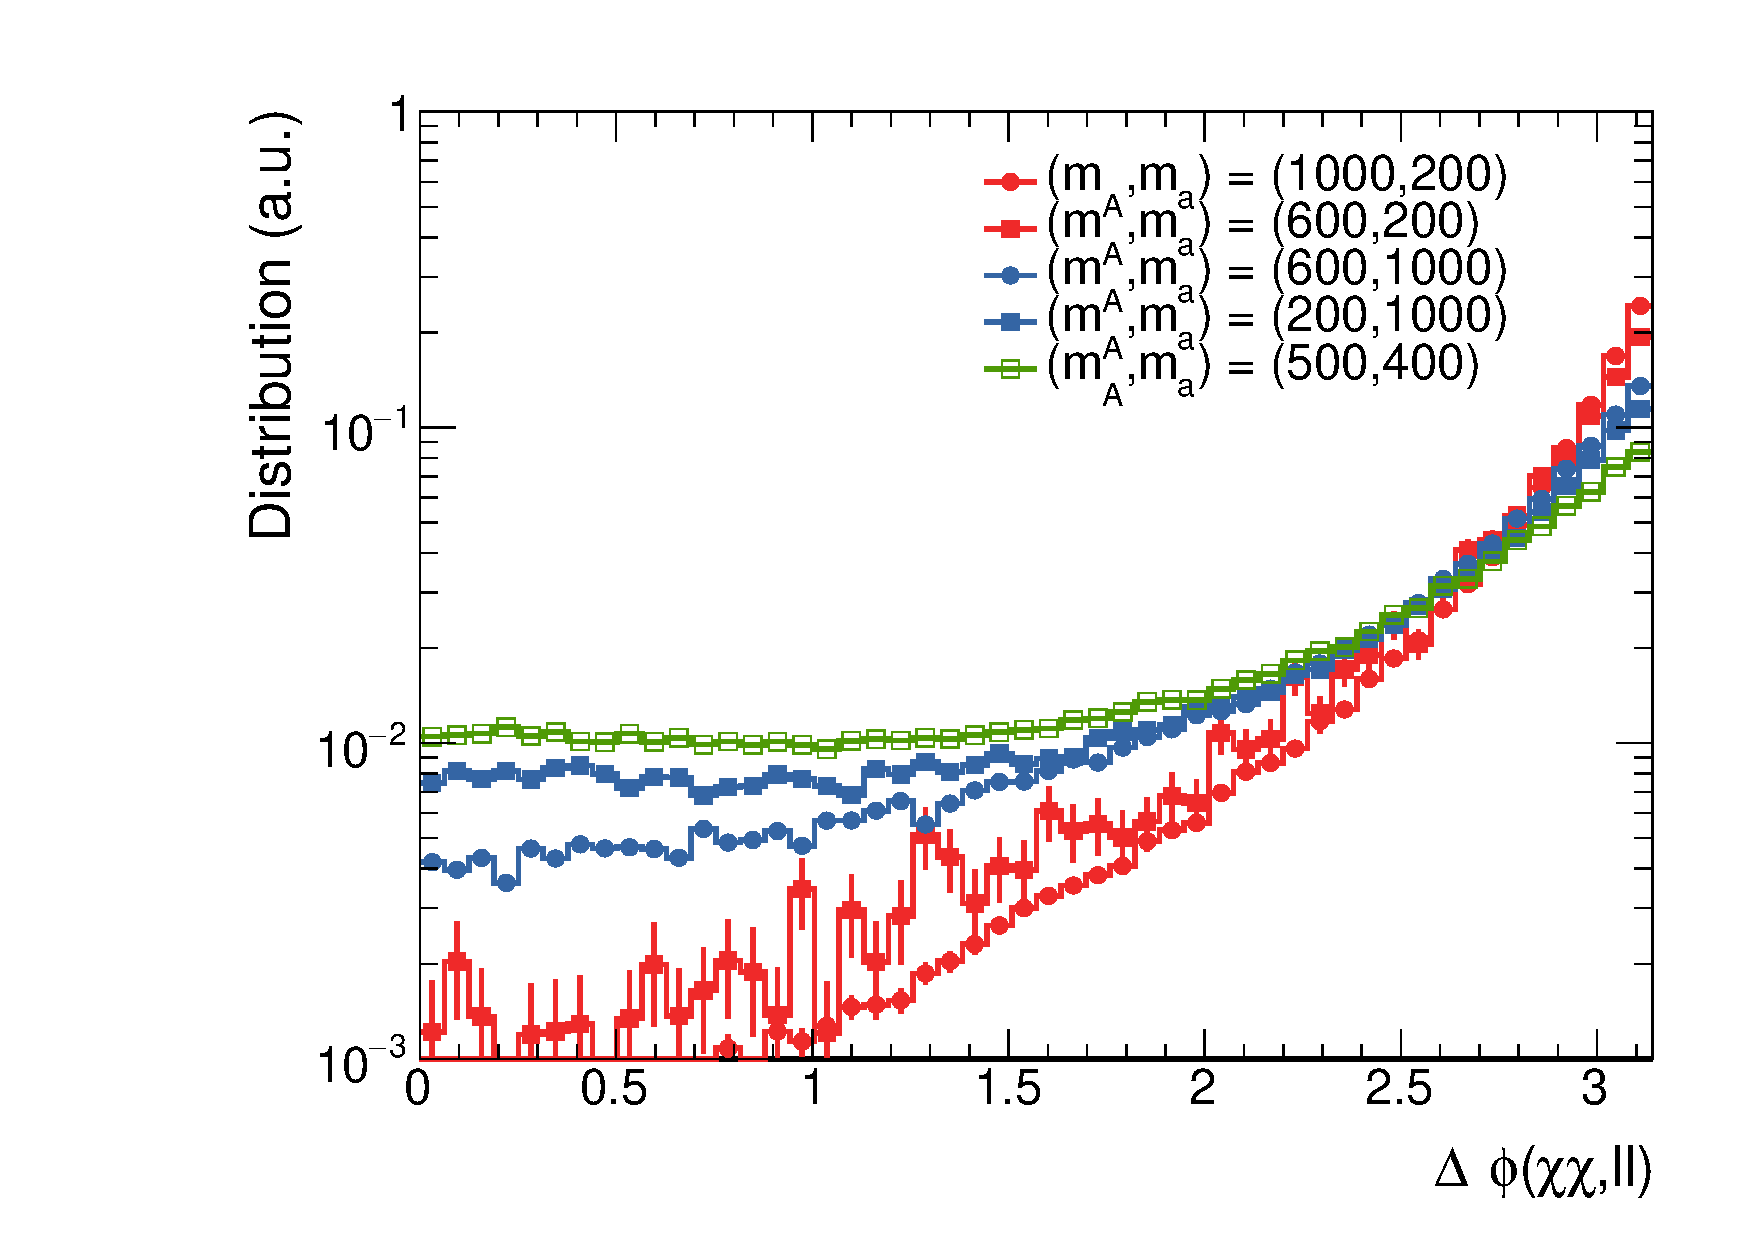
\includegraphics[width=0.45\textwidth]{texinputs/04_grid/figures/monoz/leptonic/presel_h_dphi_met_ll.pdf}
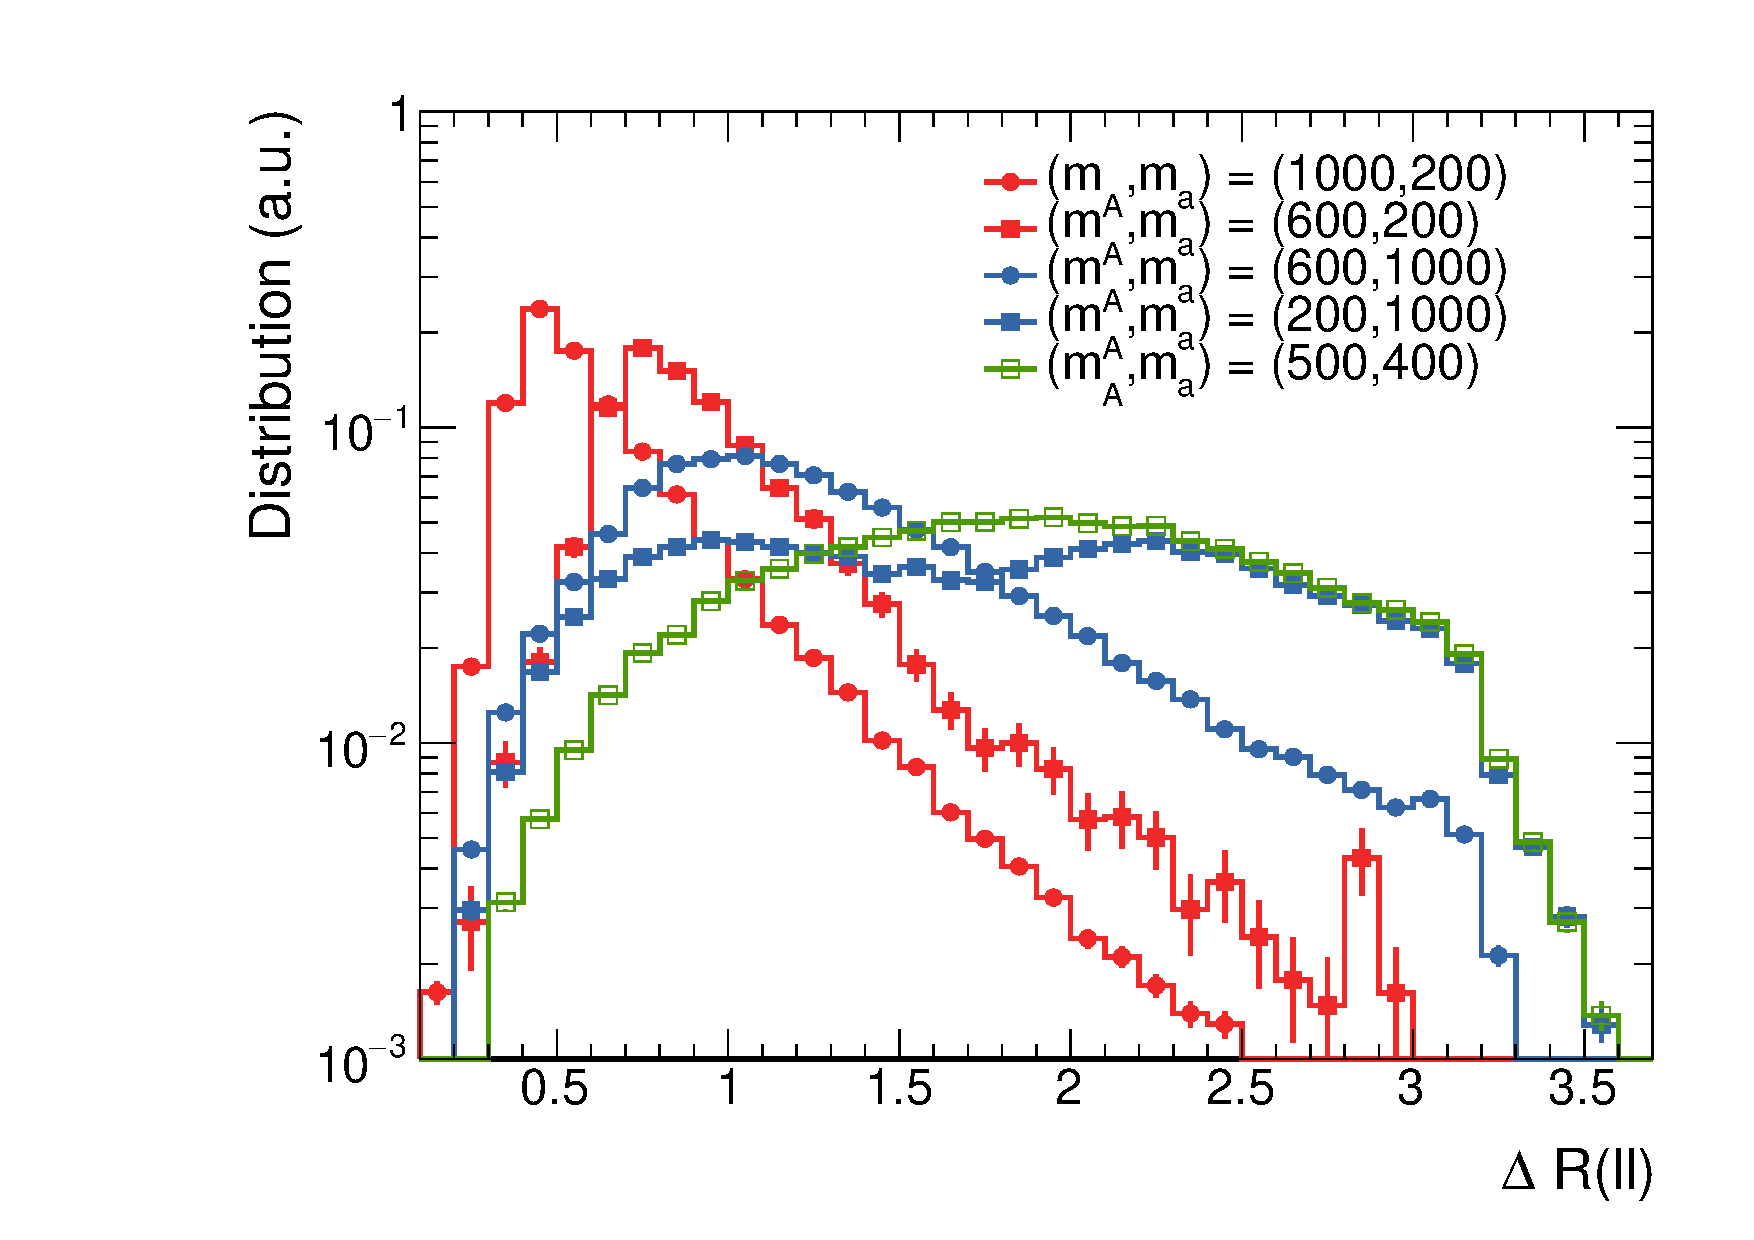
\includegraphics[width=0.45\textwidth]{texinputs/04_grid/figures/monoz/leptonic/presel_h_dr_ll.pdf}
\caption{Distributions of the main selection variables after preselection: \pt balance (top panel), $\Delta\Phi$ (middle) and $\Delta R$ (bottom). The shown parameter points illustrate the different qualitative behavior in the three different mass regions. }
\label{fig:monoz_kin_presel}
\end{figure}

